\begin{table*}
\centering
\caption{ORES wp10 fitness statistics. The fitness statistics of ORES ``wp10'' model based on 10-fold cross-validation are shown in table format.  Note that ``within-1'' accuracy represents the per-class accuracy measure where being off by one is considered a successful prediction.  The overall accuracy is 62.9\% and the within-1 accuracy is 90.7\%.  These figures compare favorably to \protect\cite{wang15success} of 58.2\% and 89.5\% respectively.  I've included the ROC-AUC metric to demonstrate that the probability estimates made by the model are generally useful.  As in \protect\cite{wang15success}, I also find that B- and C-class show lower overall fitness than other classes.}
\begin{tabular}{|c|l|l|l||l|l|l|l|l|l|} \hline
& n & ROC-AUC & acc (within-1) & ~Stub & ~Start & ~C & ~B & ~GA & ~FA \\ \hline 
Stub & 4968 & 98.5\% & 85.5\% (99.2\%)
& \cellcolor{green!25}4247
& \cellcolor{yellow!25}685 & 27 & 9 & 0 & 0 \\ \hline
Start & 4982 & 91.2\% & 64.3\% (91.5\%)
& \cellcolor{yellow!25}600
& \cellcolor{green!25}3205
& \cellcolor{yellow!25}754 & 358 & 58 & 7 \\ \hline
C & 4994 & 86.6\% & 48.9\% (86.1\%) & 44
& \cellcolor{yellow!25}870
& \cellcolor{green!25}2443
& \cellcolor{yellow!25}986 & 558 & 93 \\ \hline
B & 4990 & 84.1\% & 40.3\% (79.8\%) & 51 & 617
& \cellcolor{yellow!25}1258
& \cellcolor{green!25}2012
& \cellcolor{yellow!25}710 & 342 \\ \hline
GA & 5000 & 92.1\% & 62.7\% (93.3\%) & 1 & 19 & 313
& \cellcolor{yellow!25}304
& \cellcolor{green!25}3135
& \cellcolor{yellow!25}1228 \\ \hline
FA & 4454 & 96.1\% & 77.4\% (94.4\%) & 5 & 2 & 23 & 220
& \cellcolor{yellow!25}757
& \cellcolor{green!25}3447 \\ \hline
\end{tabular}
\label{tab:fitness_statistics}
\end{table*}

In order to enable better understanding of the dynamics of article quality in Wikipedia, I sought to develop a method that would allow for granular analysis of the quality level of articles.  Warncke-Wang et al.'s ``actionable'' modeling strategy seems particularly suitable to the task due to the high level of fitness they demonstrate (matching Wikipedians' own assessments) and its reliance on characteristics of the text content of the article (as opposed to external characteristics).  I worked with Dr. Warncke-Wang to re-implement this model in the ORES system\footnote{The Objective Revision Evaluation System is a machine prediction platform used by Wikipedians to detect vandalism, measure article quality, and automate other useful activities in Wikipedia. See \url{https://meta.wikimedia.org/wiki/ORES}} and to implement a few minor improvements since he and his collaborators last published about improvements to the model~\cite{wang15success}.  I used the related open dataset~\cite{wang15english} of assessments to train and test this model.  For a full specification of the features used in prediction including scaling and controlling features, see the code~\footnote{\url{https://github.com/wiki-ai/wikiclass/blob/950f693d789f8512e30f483f18e2d13483d13749/wikiclass/feature_lists/enwiki.py}}.  ORES currently uses a GradientBoosting algorithm with estimators=700, max-depth=7, max-features=log2, and loss=deviance~\footnote{\url{http://pythonhosted.org/revscoring/revscoring.scorer_models.html\#revscoring.scorer_models.GradientBoosting}}.  Table \ref{tab:fitness_statistics} presents the overall prediction fitness of the re-implemented model.

\begin{figure}[htbp]
	\makebox[\columnwidth]{\hrulefill}{
	\small
	\begin{verbatim}
"prediction": "GA",
"probability": {
  "Stub": 0.0019,
  "Start": 0.0132,
  "C": 0.1252,
  "B": 0.2090,
  "GA": 0.3345,
  "FA": 0.3162
}
	\end{verbatim}
	\hrule
	\normalsize}
	\caption{Quality prediction for Murie Curie. The article quality prediction of a revision of the article ``Murie Curie'' saved on April 4th, 2017 is presented.  See \url{https://ores.wikimedia.org/v2/scores/enwiki/wp10/773753742}. }
	\label{fig:murie_curie_prediction}
\end{figure}

\leadin{Modeling quality changes.} I hypothesized that, at a large enough timescale, this ``actionable model'' would be able to track \emph{quality dynamics} -- the changes in article quality over time.  After all, if the model is able to match Wikipedians' assessments, it should also be able to fill in the gaps between assessments as well.  I suspected that a large timescale that covered several revisions would be necessary for measuring article quality dynamics accurately because it takes time for Wikipedia's counter-vandalism systems to work.  \emph{I.e.} vandalism and other damaging edits to an article might also change the features extracted favorably since they are arguably quite basic (\emph{e.g.} \emph{number of headers} and \emph{number of image links} -- see \cite{wang13tell}).  It would be inappropriate to consider such an edit to have increased the quality level of the article.  By waiting a substantial time period between automatic quality predictions, Wikipedians' natural quality control processes can run their course.

There are two reasons why I have concluded that this strategy is working in practice:  (1) I performed a set of basic spot-checks on hand-picked articles focusing on substantial quality changes and (2) I released this prediction model publicly 2 years ago and since then many users have told my collaborators and I that they find it to be effective and useful for supporting their work.  I was actually quite surprised to find that the large timescale between assessments seems to not be necessary at all.  Users report that the model is accurate and useful even when used to score every version of a page and that, in general, vandalism appears as either no change or a decrease in article quality as intended~\cite{ross2016visualizaing}.

One additional request that I received from Wikipedia editors was to provide a mechanism for getting between-class quality predictions.  So I developed a basic strategy that I refer to as the \emph{weighted sum} of class predictions.  I assume that the ordinal article quality scale developed by Wikipedia editors is roughly cardinal and evenly spaced.  To arrive at the \emph{weighted sum} measurement, multiply the prediction probability for each class by an enumeration of ordered classes starting at zero (0) for Stub and ending at five (5) for FA.

\begin{equation} \label{eq:weighted_sum}
\begin{split}
\text{weighed sum} = \sum_{c \in C}{I(c)P(c)}
\end{split}
\end{equation}
This equation weighs each step in quality the same by multiplying the index of the class $I(c)$ by the prediction probability for that class $P(c)$.

When the model predicts that a version of an article is a Stub with 100\% confidence, this \emph{weighted sum} would be 0.  If the prediction were split 50\% Start and 50\% C, the weighted sum would be 1.5.  The \emph{weighted sum} of the prediction demonstrated in figure~\ref{fig:murie_curie_prediction} would be 3.8096 -- slightly on the B side of GA-class.  Again, my own spot checking and ORES' users confirm that this appears to be useful and consistent when applied to the history of articles.

Once I had concluded that the model operated consistently over time, I worked with my collaborators to generate a dataset that contains a predicted quality level for all articles in English Wikipedia at a monthly interval (~600m article-month predictions).  This dataset~\cite{halfaker16monthly} contains the highest probability quality class (``prediction'') as well as the \emph{weighted sum} measurement for each article-month (``weighed\_sum'').

\begin{figure*}[p]
\centering
\begin{subfigure}[t]{.95\columnwidth}
  \centering
  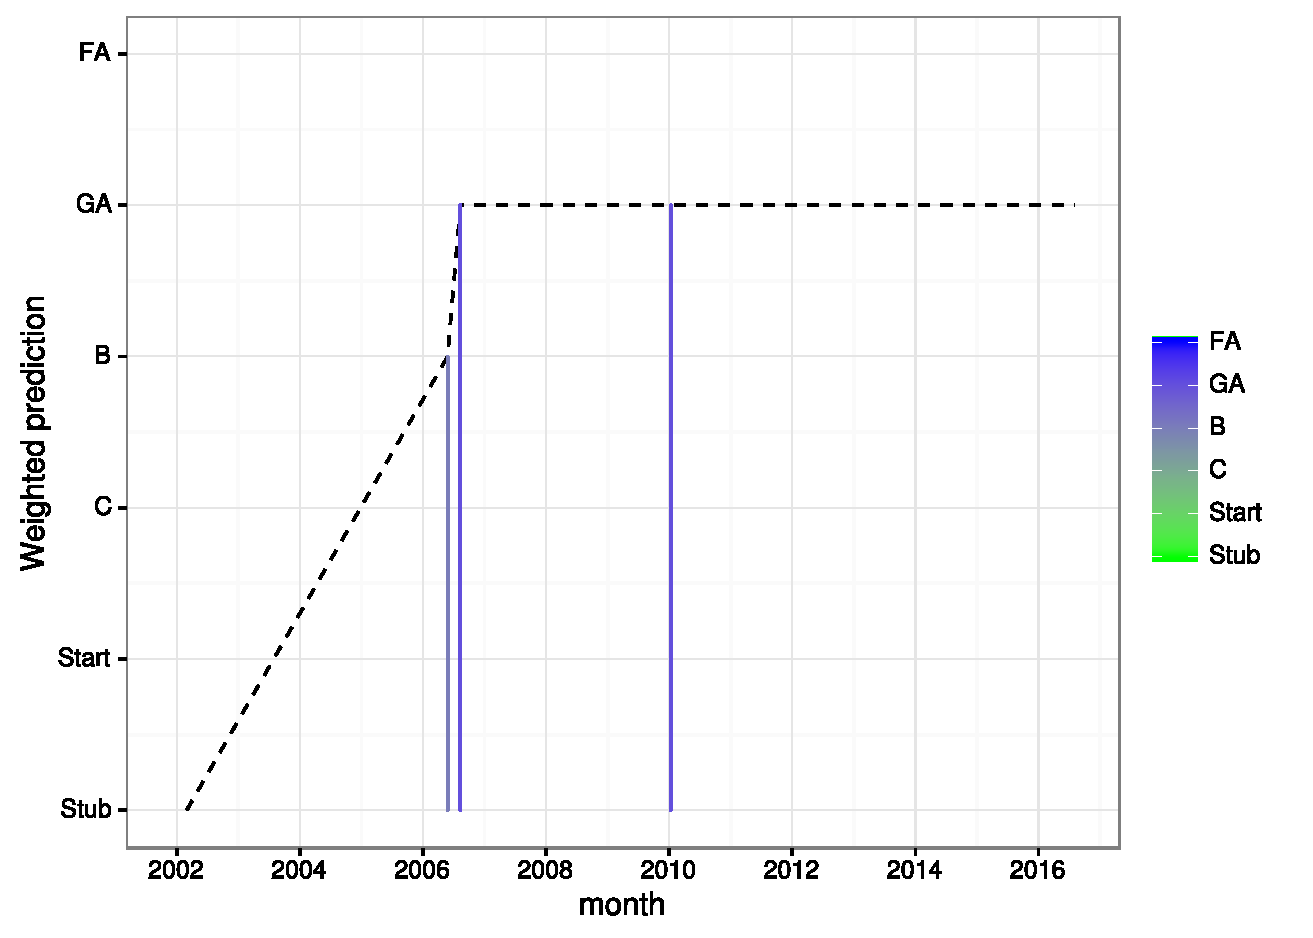
\includegraphics[width=.90\columnwidth]{figures/biology_monthly_assessments}
  \caption{Biology's assessments.  The 3 manual assessments of the quality of Biology are plotted over time with a dashed line connecting them.}
  \label{fig:empirical_biology}
\end{subfigure}~~
\begin{subfigure}[t]{.95\columnwidth}
  \centering
  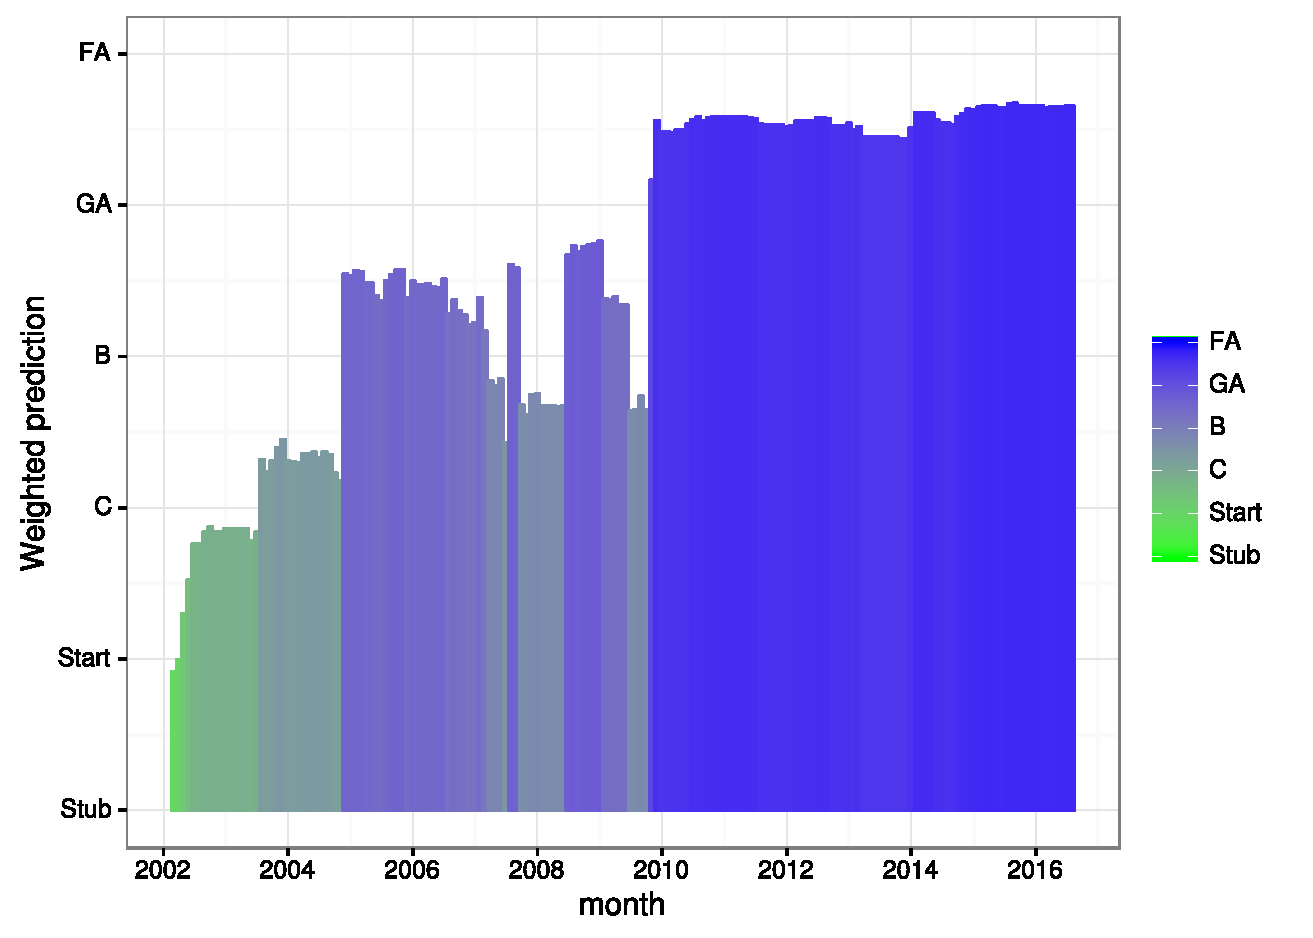
\includegraphics[width=.90\columnwidth]{figures/biology_monthly_wp10}
  \caption{Biology's predicted quality.  The \emph{weighted sum} prediction for the article Biology as of the last revision at the beginning of each month is plotted.}
  \label{fig:predicted_biology}
\end{subfigure}
\caption{Comparing assessments to predicted quality for Wikipepdia's article titled ``Biology''.  Note how~\ref{fig:predicted_biology} shows much more nuanced detail about the development of the article over time than~\ref{fig:empirical_biology}.}
\label{fig:empirical_and_predicted_biology}
\end{figure*}


\leadin{Aggregated quality measures.} Using this dataset, we can move up a level from articles and assess the quality of Wikipedia at an aggregate level -- as a whole or across interesting cross-sections.  I employed two aggregation strategies for comparing the quality of article aggregates: the \emph{mean weighted sum}, and proportions of articles falling into each predicted class.  In order to give these measurements a useful denominator I use the total number of articles in the aggregate as of the the most recent month in the dataset.  Since the number of articles is clearly monotonically increasing (article creations always outnumber deletions), the count in the last month is always the \emph{max} number of articles for any month in the cross-section.  Assuming that a Stub (the lowest quality class) is substantially more useful than no article at all so I assign a zero (0) \emph{weighted sum} for all articles that have yet to be created in a particular month and increment the weighed sum for articles that exist by one (1) when generating the aggregate weighed some.  So if all articles were empty (like in the month before Jan 2001 -- inception of Wikipedia), the \emph{mean weighted sum} is zero.  If all articles were predicted to be 100\% FA class, the \emph{mean weighted sum} would be 6.

These assumptions are bold and clearly provide an incomplete view of the reality of Wikipedia.  \emph{E.g.} if one were to draw a cross section of Wikipedia that included only one FA-class article, that cross-section would get the maximum \emph{mean weighted sum}.  If in a following month, a Stub article were created, then the \emph{mean weighted sum} would decrease even though there is more useful content.  However, because this measure uses the number of articles in the last month as the denominator for all months, the \emph{mean weighted sum} would also decrease historically, so this assumption is somewhat fair.  Still, this assumption implies that Wikipedia will get no new articles after the date at which the dataset is generated.  I feel that this is acceptable for comparing cross-sections/aggregates that have more than a trivial number of articles and that are also generated using normal Wikipedian processes.  I'll discuss this complicated problem and propose some solutions for addressing it for section~\ref{sec:future_work}.  For the purposes of the demonstration analysis, I encourage you, dear reader, to judge this analysis by it's interest as a demonstration of the novel measurement capabilities and how this method enables us to visualize shifts in quality over time.
